\tikzset{every picture/.style={line width=0.75pt}} %set default line width to 0.75pt        

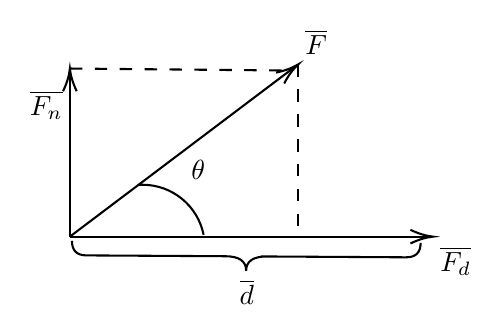
\begin{tikzpicture}[x=0.75pt,y=0.75pt,yscale=-1,xscale=1]
%uncomment if require: \path (0,300); %set diagram left start at 0, and has height of 300

%Straight Lines [id:da3935293311213366] 
\draw    (238,106) -- (346.4,24.2) ;
\draw [shift={(348,23)}, rotate = 142.96] [color={rgb, 255:red, 0; green, 0; blue, 0 }  ][line width=0.75]    (10.93,-3.29) .. controls (6.95,-1.4) and (3.31,-0.3) .. (0,0) .. controls (3.31,0.3) and (6.95,1.4) .. (10.93,3.29)   ;
%Straight Lines [id:da4139500414390731] 
\draw    (238,106) -- (411,106) ;
\draw [shift={(413,106)}, rotate = 180] [color={rgb, 255:red, 0; green, 0; blue, 0 }  ][line width=0.75]    (10.93,-3.29) .. controls (6.95,-1.4) and (3.31,-0.3) .. (0,0) .. controls (3.31,0.3) and (6.95,1.4) .. (10.93,3.29)   ;
%Shape: Brace [id:dp7665000243293123] 
\draw   (239,108) .. controls (238.97,112.67) and (241.29,115.01) .. (245.96,115.04) -- (312.96,115.44) .. controls (319.63,115.48) and (322.95,117.83) .. (322.92,122.5) .. controls (322.95,117.83) and (326.29,115.52) .. (332.96,115.56)(329.96,115.54) -- (399.96,115.96) .. controls (404.63,115.99) and (406.97,113.67) .. (407,109) ;
%Straight Lines [id:da5936849259351216] 
\draw  [dash pattern={on 4.5pt off 4.5pt}]  (348,23) -- (348,106) ;
%Straight Lines [id:da5595911093922712] 
\draw  [dash pattern={on 4.5pt off 4.5pt}]  (238,25) -- (346,26) ;
%Straight Lines [id:da7278258054036395] 
\draw    (238,106) -- (238,27) ;
\draw [shift={(238,25)}, rotate = 90] [color={rgb, 255:red, 0; green, 0; blue, 0 }  ][line width=0.75]    (10.93,-3.29) .. controls (6.95,-1.4) and (3.31,-0.3) .. (0,0) .. controls (3.31,0.3) and (6.95,1.4) .. (10.93,3.29)   ;
%Shape: Arc [id:dp3843396654817173] 
\draw  [draw opacity=0] (271.07,81.06) .. controls (271.71,81.02) and (272.35,81) .. (273,81) .. controls (287.55,81) and (299.69,91.36) .. (302.42,105.12) -- (273,111) -- cycle ; \draw   (271.07,81.06) .. controls (271.71,81.02) and (272.35,81) .. (273,81) .. controls (287.55,81) and (299.69,91.36) .. (302.42,105.12) ;  

% Text Node
\draw (323.22,125.4) node [anchor=north] [inner sep=0.75pt]    {$\overline{d}$};
% Text Node
\draw (350,19.6) node [anchor=south west] [inner sep=0.75pt]    {$\overline{F}$};
% Text Node
\draw (236,34.4) node [anchor=north east] [inner sep=0.75pt]    {$\overline{F_{n}}$};
% Text Node
\draw (295,67.9) node [anchor=north west][inner sep=0.75pt]    {$\theta $};
% Text Node
\draw (415,109.4) node [anchor=north west][inner sep=0.75pt]    {$\overline{F_{d}}$};


\end{tikzpicture}
